\documentclass[a4paper]{article}
\usepackage[pdftex]{graphicx}
\usepackage[utf8]{inputenc}
\usepackage{enumerate}
\usepackage{siunitx}
\sisetup{locale=DE} 
\usepackage{icomma}
\usepackage{amssymb}
\usepackage{tikz}
\usepackage{href-ul}
\hypersetup{
	colorlinks=true,
	linkcolor=blue,
	urlcolor=blue}
\usepackage{geometry}
\geometry{a4paper, top=15mm, left=15mm, right=15mm, bottom=15mm,
	headsep=10mm, footskip=12mm}

\begin{document}
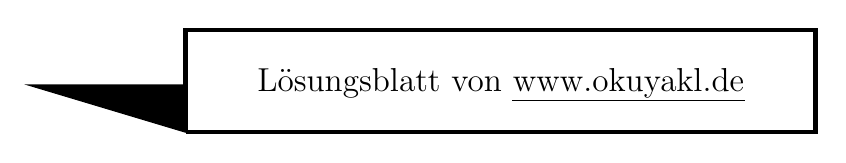
\begin{tikzpicture}(10,3)
	\draw[ultra thick](2,0) --(10,0) -- (10,1.3) --(2,1.3) -- (2,0);
	\draw[fill=black](2,0)-- (0,.6) -- (2,.6) -- (2,0);
	\node at (6,.6) {\large Lösungsblatt von \href{https://www.okuyakl.de}{www.okuyakl.de}};
\end{tikzpicture}
\vspace{0.5 cm}


\noindent{\bf Aufgabe 1.}\\
\renewcommand{\arraystretch}{3}
\begin{tabular}{|p{3.5 cm}|p{3.5 cm}|p{10 cm}|}
	\hline
	Physikalische Größe &  Formel & Einheit \\
	\hline
	Kraft & $F = m \cdot a $ & 1 Newton $\left(\SI{1}{\newton} = \SI{1}{\kilogram \cdot {\meter \over \second^2}}\right)$\\
	\hline
	Druck & $p = {F  \over A}$ & 1 Pascal $\left(\SI{1}{\pascal} =\SI{1}{\newton\over\meter^2}=\SI{1}{\kilogram\over{\meter\second^2}}\right)$\\
	\hline
	Arbeit & $ W = F \cdot s $ & 1 Newtonmeter = 1 Joule $\left(\SI{1}{\joule} =\SI{1}{\newton\meter} = \SI{1}{\kilogram \cdot { \meter^2 \over \second^2}}\right)$\\
	\hline
	Potentielle Energie & $ E =  m \cdot g \cdot h $ & 1 Newtonmeter = 1 Joule $\left(\SI{1}{\joule} =\SI{1}{\newton \meter}=\SI{1}{\kilogram \cdot {\meter^2 \over \second^2}}\right)$\\
	\hline
	Leistung & $P = {W \over t}\quad (=U \cdot I)$ & 1 Watt = $\left( \SI{1}{\watt} =\SI{1}{\joule\per \second} =\SI{1}{\kilogram\cdot {\meter^2 \over \second^3}} \right) $\\
	\hline
\end{tabular}
\vspace{1 cm}

\noindent{\bf Aufgabe 2.}\\
Die Dichte $\varrho_g$ des Gases ist dessen Masse, geteilt durch das Volumen:
$$\varrho_g={m \over V} = {\SI{2,2}{\kilogram}\over\SI{3,1}{\meter^3}}= \SI{0,71}{\kilogram \over \meter^3}$$
Die gefundene Dichte ist geringer als diejenige von Luft, darum erfährt ein mit diesem Gas gefüllter Luftballon eine Auftriebskraft, sodass er, wenn seine Hülle nicht zu schwer ist, fliegen kann. 
\vspace{0.5 cm}

\noindent{\bf Aufgabe 3. a)}\\
Drücke misst man allgemein mit einem Manometer.
\vspace{0.5 cm}

\noindent{\bf Aufgabe 3. b)}\\
Den Luftdruck misst man mit einem Barometer.
\vspace{0.5 cm}

\noindent{\bf Aufgabe 4. a)}\\
Der Luftdruck ist abhängig vom Wetter und von der Höhe.
\vspace{0.5 cm}

\noindent{\bf Aufgabe 4. b)}\\
Der Schweredruck im Wasser nimmt mit der Tiefe alle 10 Meter um eine Atmosphäre ($\approx \SI{1000}{\hecto\pascal}$) zu.
\vspace{0.5 cm}

\noindent{\bf Aufgabe 4. c)}\\
Kraft = Druck mal Fläche:
$$ F = p\cdot A = \SI{8e6}{\newton\over \meter^2}\cdot {600 \over 10000}~\SI{}{\meter^2} = \SI{480000}{\newton}=\SI{480}{\kilo\newton}$$
Dies entspricht einer Gewichtskraft, die eine $\SI{48}{\tonne}$ schwere Flüssigkeitssäule besitzt.
\vspace{0.5 cm}

\noindent{\bf Aufgabe 4. d)}\\
Der Druck von $\SI{8}{\mega\pascal}$ ist das 80-Fache des normalen Luftdrucks von $\SI{1000}{\hecto\pascal}=\SI{0,1}{\mega\pascal}$. Also befindet sich nach der Merkregel aus 4. b) das U-Boot in $80\cdot 10~\SI{}{\meter}=\SI{800}{\meter}$ Tiefe.  

\begin{center}
	\includegraphics[width=7 cm]{../../viecher/endcomic.pdf}
	
	Hier geht es zurück zum \href{https://www.okuyakl.de/phys/p8druL108/aa108.pdf}{Aufgabenblatt}
\end{center}

\end{document}